\documentclass[a4paper, 12pt]{article}

\usepackage[utf8]{inputenc} % POUR MODIFIER : ALLER DANS PREFERENCE TEXSHOP
\usepackage[T1]{fontenc}
\usepackage[francais]{babel}
\usepackage{verbatim}
\usepackage{moreverb}
\usepackage{algorithm, algpseudocode}%Meilleur que listing???

\usepackage{listings} % Pour écrire algo

\usepackage{listingsutf8}

%Paramètrage avec : 
\renewcommand{\lstlistingname}{Interface}
%\lstset{
%basicstyle=\footnotesize,    % taille de la police du code
%numbers=left,   % placer le numéro de chaque ligne à gauche (left) 
%numberstyle=\normalsize,    % taille de la police des numéros
%numbersep=8pt,  % distance entre le code et sa numérotation
%}
\lstset{
language=c++,        % choix du langage de programmation 
  frame=single,
  basicstyle=\small\normalfont\sffamily,    % the size of the fonts that are used for the code
  stepnumber=1,                           % the step between two line-numbers. If it is 1 each line will be numbered
 % numbersep=10pt,                         % how far the line-numbers are from the code
  tabsize=1,                              % tab size in blank spaces
  breaklines=true,                        % sets automatic line breaking
  captionpos=t,                           % sets the caption-position to top
  mathescape=true,
  %stringstyle=\color{white}\ttfamily, % Farbe der String
  showspaces=false,           % Leerzeichen anzeigen ?
  showtabs=false,             % Tabs anzeigen ?
  xleftmargin=17pt,
  framexleftmargin=17pt,
  framexrightmargin=17pt,
  framexbottommargin=5pt,
  framextopmargin=5pt,
  showstringspaces=false,
  inputencoding=utf8,
  extendedchars=true,
  literate=%
            {é}{{\'{e}}}1
            {è}{{\`{e}}}1
            {ê}{{\^{e}}}1
            {ë}{{\¨{e}}}1
            {û}{{\^{u}}}1
            {ù}{{\`{u}}}1
            {â}{{\^{a}}}1
            {à}{{\`{a}}}1
            {î}{{\^{i}}}1
            {ô}{{\^{o}}}1
            {ç}{{\c{c}}}1
            {Ç}{{\c{C}}}1
            {É}{{\'{E}}}1
            {Ê}{{\^{E}}}1
            {À}{{\`{A}}}1
            {Â}{{\^{A}}}1
            {Î}{{\^{I}}}1  
 }

\usepackage{graphicx} % Pour les images 
\usepackage{appendix} % Pour annexes

\usepackage{lmodern}
\usepackage{fancyhdr}

\usepackage[hidelinks]{hyperref} 
\usepackage{url} % Pour écrire des adresses cliquables.
\usepackage[top=2cm, bottom=2cm, left=2cm, right=2cm]{geometry} % Les marges.
\renewcommand{\thesection}{\arabic{section}}

\usepackage{amsmath}
\usepackage{amssymb}
\usepackage{mathrsfs}

\pagestyle{fancy}

\renewcommand{\headrulewidth}{0pt} % Pour enlever la ligne horizontale en haut
\renewcommand{\footrulewidth}{1pt}
\fancyhead[L,R]{}
\fancyfoot[R]{\textbf{page \thepage}} 
\fancyfoot[L]{Rapport : Courbes de Bézier et polices de caractères}
\fancyfoot[C]{}  

\begin{document}

\begin{titlepage}
			
\includegraphics[scale=0.25]{Images/logo_ENSIIE.png} 
			\begin{center}
				\vspace*{6cm}
				{ \huge Rapport Projet PAP \\ \vspace*{2cm}
				\textbf{Courbes de Bézier et polices de caractères} \\
				}
			\vspace*{2cm}
				\begin{center} \large
					\textsc{XU} \textsc{Kevin}\\
					\textsc{LI} \textsc{Ziheng}
				\end{center}
				\begin{minipage}{0.4\textwidth}
				\end{minipage}
				{\large 13 janvier 2019}
			\end{center}
	\end{titlepage}
	
	%Sommaire
	\renewcommand{\contentsname}{Sommaire} 
	{\setlength{\baselineskip}{1.2\baselineskip}
\tableofcontents\par} %RAJOUTER ESPACE ENTRE LIGNE
		
	\addcontentsline{toc}{part}{Préambule} %Ajouter un lien
	\newpage
	\vspace*{3cm} 
	\paragraph{\Huge{Préambule}}

	\paragraph{}
	L'objectif de ce projet est de réalisé des polices de caractères en utilisant des courbes de Bézier. Le programme est implémenté en C++, sans l’aide d’une quelconque bibliothèque extérieure au C++.
	Trois polices de caractères pour les lettres de l’alphabet en majuscule et sans sérif ont été créée : 	
	
	\begin{enumerate}
		\item La première police correspond aux glyphes décrivant le contour du caractère en noir dans un bitmap (rectangle de pixels blancs et noirs, les pixels noirs étant donc le contour du caractère). 
		\item La deuxième police est la première police mais avec l’intérieur des caractères rempli en noir, toujours dans un bitmap. 
		\item La troisième police est la deuxième police mais avec un contour rouge de deux pixels à l’extérieur du caractère. Ce style de police est très utile pour les sous-titrages des films, pour pouvoir toujours lire le sous-titre quelque soit la scène du film. 
 	\end{enumerate}

	Pour fournir les images png de chaque caractère des différentes polices, nous avons utilisé la bibliothèque libpng.
\newline

Nous allons tout d’abord présenter les classes de notre programme. Puis nous évoquerons les objectifs, problèmes rencontrés et les solutions trouvés pour chacune des classes.


	
	\newpage

\section{Les classes (Diagramme UML)}			
\subsection{Diagramme UML}

\section{Point - Classe \texttt{Point}}	
\subsection{Objectifs}
	Tout d'abord, sachant qu'une courbe de Bézier est formée par plusieurs points, il faut avoir une classe définissant un point sur un système de coordonnées dans un plan. Le but de cette classe est alors de définir les point des courbes de Bezier que l'on va tracer. En outre, il faut aussi pouvoir avoir la possibilité de dessiner des points de différentes couleurs.
	
\subsection{Solution}
Une instance de la classe \texttt{Point} a 3 attributs : 
\begin{itemize}
\item La coordonnée $x\_$
\item La coordonnée $y\_$
\item Un tableau $color\_$ contenant les niveaux de Rouge, Vert et de Bleu (allant de 0 à 255). 
\end{itemize}
Cette classe contient aussi les getters et setters pour ces attributs.

\section{Les image - Classe \texttt{Image}}	
\subsection{Objectifs}
Afin de pouvoir fournir les images PNG de chaque caractère, nous avons décidé de créer une classe \texttt{Image}. Cette classe s'occupe de toute la gestion des images comme la création et la modification des pixels sur l'image.

\subsection{Solution et Réalisation}
Pour réaliser cette classe, on a utiliser la bibliothèque \textbf{libpng}. Cette dernière nous permet de créer des images et de modifier les pixels avec la couleur que l'on souhaite.
Elles contient notamment les méthodes permettant de dessiner des \texttt{Point} et des \texttt{BezierCurve}.\\

Dans le constructeur de la classe, on a décidé que l'image créée aura un fond blanc par défaut. 

% \newpage

\section{Courbes de Bézier - Classe \texttt{BezierCurve}}	
\subsection{Objectifs	}
Cette classe est l’une des classes les plus importantes du programme. Afin de tracer les différentes courbes d’un caractère, nous devons implémenté une classe permettant de calculer les points à tracer afin d'obtenir des courbes de Bézier. En effet, chaque caractère est composé de courbes de Bézier linéaire et/ou quadratique.

\subsection{Solution et Réalisation}
La classe contient deux attributs : 
\begin{itemize}
	\item Un vecteur de \texttt{Point} $points\_$ qui contient les points de contrôles de la courbe de Bézier à tracer
 	\item Un réel $step\_$ qui correspond à la précision de l'algorithme de Casteljau
\end{itemize}
\vspace*{0.5cm}
Nous disposons de deux méthodes primordiales pour créer les courbes de Bézier :
\begin{itemize}
\item \texttt{void addPoints(Point)} : Cette méthode permet d'ajouter un point de contrôle à la courbe de Bézier
\item \texttt{void clearPoints()}: Cette méthode permet de supprimer tous les points de contrôles de la courbe de Bézier.
\end{itemize}
% \vspace{0.5cm}

\subsubsection{Algorithme de Casteljau}
Pour tracer une courbe de Bézier, nous n'avons pas utilisé la formulation mathématique comme présentée dans le sujet. En effet, l’algorithme de Casteljau développé par Paul de Casteljau permet de réaliser cela en utilisant une approche récursif pour approximer les courbes de Bézier.

Le principe de l'algorithme est de construire récursivement un ensemble de barycentres se rapprochant au fur et à mesure de la courbe de Bézier. L'algorithme s'arrête alors lorsque toutes les distances entre deux points consécutifs sont assez petites.
Nous avons imposé une valeur du paramètre $step\_ = 0.000001$ pour les calculs de barycentre.
% \vspace*{0.5cm}

\begin{algorithm}
	\caption{\texttt{getCasteljauPoint}}
		\begin{algorithmic}[1]
		\Require $c \in \mathbb{N}$, $index \in \mathbb{N}, t \in \mathbb{R}^{*}$, $points$ A vector which contains the control points of the Bezier Curve
		\Ensure The Point computed with the De Casteljau's algorithm
		\Function{getCasteljauPoint}{$c$, $index$, $t$, $points$}
		\If{ c = 0 }
			\State \Return points[index] 
		\EndIf
		\State Set a Point in $P1$ to \texttt{getCasteljauPoint(}$c-1$, $index$, $t$, $points$\texttt{)} 
		\State Set a Point in $P2$ to \texttt{getCasteljauPoint(}$c-1$, $index+1$, $t$, $points$\texttt{)} 
		\State Set a Point in $P$ with $x = (1-t) \times (x \; of \; P1) + t \times (x \; of \; P2)$ and $y = (1-t) \times (y \; of \; P1) + t \times (y \; of \; P2)$
		\State \Return $P$
		\EndFunction
		\end{algorithmic}
\end{algorithm}

\begin{algorithm}
	\caption{\texttt{getCurvePoints}}
		\begin{algorithmic}[1]
		\Require $points$ The control points of the Bezier Curve, $step$ The parameter of the barycenter
		\Ensure A vector $Res$ of Points which picture the Bezier Curve
		\Function{getCurvePoints}{$points$, $step$}
		\State Set an empty vector $Res$ of Points
		\State Set $size$ to the size of the vector $points$
		\For{$t = 0$ to $1$ with a step of $step$}
			\State Add to the vector $Res$ the Point : \texttt{getCasteljauPoint(}$size-1$, $0$, $t$, $points$\texttt{)} 
		\EndFor
		\State \Return $Res$
		\EndFunction
		\end{algorithmic}
\end{algorithm}

Cette algorithme nous permet de tracer des courbes de Bézier linéaires et quadratiques. Mais on peut aussi tracer des courbes avec plus de trois points de contrôles comme des courbes de Bézier cubiques ou plus. Cependant, dans le cadre de notre projet, nous avons seulement utiliser l'algorithme pour trois points de contrôles au plus seulement.

\subsubsection{Résultats et Problèmes rencontrés}
Pour certaines courbes de Bézier, on a rencontré quelques problèmes. En raison des erreurs d'approximations, il peut arriver que certaines courbes de Bézier présentes des pixels non reliés entre elles. Voici un exemple : 

\begin{figure}[h]
\centering
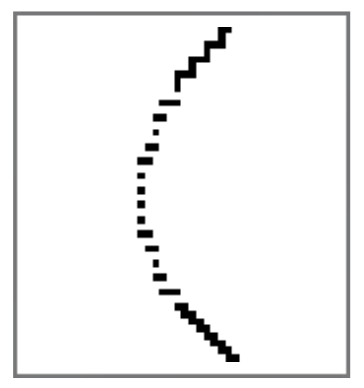
\includegraphics[scale=0.3]{Images/BezierCurbe_problem.png}
\caption{Courbe non reliée}
\label{fig1}
\end{figure}

En effet, cela est dû dans certains cas à un $step\_$ pas assez petit. Mais plus la valeur de cette variable est petite, plus le temps d’exécution sera élevé. C'est pour cela qu'on a décidé de définir $step\_ = 0.000001$ après avoir tester différentes valeurs.

\newpage
\section{Première Police - Classe \texttt{FontV1}}	
\subsection{Objectifs}
Pour réaliser la première police, on doit créer une classe qui contient les méthodes pour dessiner toutes les lettres de l'alphabet dans des images PNG. En outre, le but de la deuxième question est de remplir l'intérieur des lettres de la première question, donc il faut produire un résultat utilisable par des classes filles.

\subsection{Solution et Réalisation}
La classe \texttt{FontV1} contient alors les attributs suivants : 
\begin{itemize}
\item \texttt{img\_} Une instance de la classe \texttt{Image} sur laquelle la lettre va être dessiner de taille 500x500 pixels
\item Un entier \texttt{thickness\_}$= 20$ qui correspond à l'épaisseur des lettres que l'on souhaite. 
\end{itemize}
\vspace{0.5cm}

Tout d'abord, on a pensé à implémenter des méthodes qui génèrent les images des lettres directement quand on saisit une lettre que l'on veut l'afficher. Cependant, on s'en rendu compte que cela était impossible pour notre niveau de connaissance.

De fait, pour générer les caractères, on a implémenté 26 méthodes différentes qui tracent chacune les courbes de Bézier permettant de dessiner une lettre de l'alphabet sur l'image \texttt{img\_}. Pour certaines lettres, on a beaucoup de courbes de Bézier à tracer, donc la taille des méthodes est parfois supérieur à 50 lignes.\\

Les lettres comportant que des courbes de Bézier linéaires ont été plus faciles à tracer que celle comportant beaucoup de courbes de Bézier quadratiques. Voici quelques lettres tracées avec cette classe : 

\begin{figure}[h]
\centering
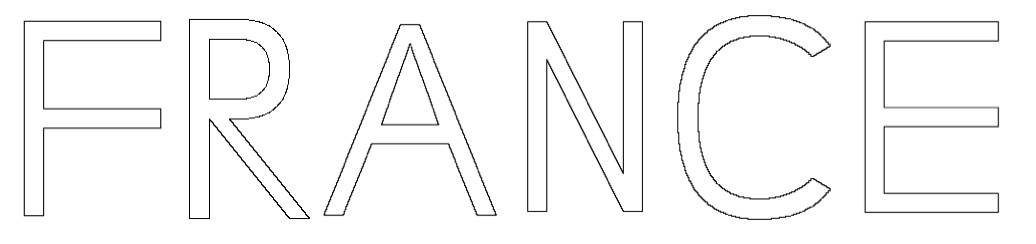
\includegraphics[scale=0.5]{Images/FRANCE_FontV1.jpeg}
\caption{Le mot FRANCE avec la police 1}
\label{fig2}
\end{figure}

\newpage
\section{Deuxième Police - Classe \texttt{FontV2}}	
\subsection{Objectifs	}
Pour générer les caractères de la deuxième police, on a créé une classe \texttt{FontV2}. Cette police est la police précédente mais avec l'intérieur des contours colorié en noir.

\subsection{Solution et Réalisation}
Au début, on a voulu remplir l'intérieur des lettres en traçant plusieurs courbes de Bézier en suivant les contours des lettres. Mais le résultat n'était pas très précis car il y avait parfois des trous blancs à l'intérieur des contours des lettres. De plus, cette méthode devait calculer plusieurs courbes de Bézier en plus de celles du contours de la lettre. Voici à quoi ressemblait notre première version de la police 2 : 

\begin{figure}[h]
\centering
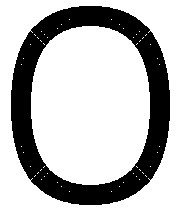
\includegraphics[scale=0.9]{Images/FontV2_O_Old.png}
\caption{Première version de la police 2}
\label{fig3}
\end{figure}

	Pour résoudre ce problème, on a utilisé l'\textbf{algorithme de remplissage par diffusion (Flood fill ou seed fill)}. Voici son pseudo-code :
 
\begin{algorithm}
	\caption{\texttt{colorInBlack}}
		\begin{algorithmic}[1]
		\Require $x \in \mathbb{N}$, $y \in \mathbb{N}$
		\Ensure Color a white area in black
		\Function{colorInBlack}{}
		\If{The coordinates $(x, y)$ are out of bounds}
			\State \Return
		\EndIf
		\If{The pixel of coordinates $(x, y)$ is white}
			\State Color the pixel of coordinates $(x, y)$ in black on the Image $img$
			\State \texttt{colorInBlack(x+1, y)} 
			\State \texttt{colorInBlack(x-1, y)} 
			\State \texttt{colorInBlack(x, y+1)} 
			\State \texttt{colorInBlack(x, y-1)} 
		\EndIf	
		\EndFunction
		\end{algorithmic}
\end{algorithm}
\newpage
La classe \texttt{FontV2} est une classe fille de la classe \texttt{FontV1}. En effet, on doit dans un premier temps faire appel à une des méthodes de la classe \texttt{FontV1} pour dessiner sur l'image les contours d'une lettre. C'est alors que par la suite on peut faire appel à l'algorithme \textbf{seed fill} en choisissant un point de départ à l'intérieur du contour de la lettre pour remplir l'intérieur de noir.\\

On obtient alors le résultat suivant pour la lettre O : 

\begin{figure}[h]
\centering

\includegraphics[scale=0.9]{Images/FontV2_O.png}
\caption{Lettre O avec la police 2}
\label{fig4}
\end{figure}

\begin{figure}[h]
\centering

\includegraphics[scale=0.5]{Images/FRANCE_FontV2.jpeg}
\caption{Le mot FRANCE avec la police 2}
\label{fig5}
\end{figure}

\newpage
\section{Troisième Police - Classe \texttt{FontV3}}		
\subsection{Objectifs}
La troisième police consiste à ajouter un contour de 2 pixels autour des contours des lettres de la deuxième police. 

\subsection{Solution et Réalisation}
La classe \texttt{FontV3} hérite de la classe \texttt{FontV2}. En utilisant cette héritage, il suffit de tracer les lettres grâce aux méthodes de la classe \texttt{FontV2}. Puis l'algorithme suivant est appliqué :   

\begin{algorithm}
	\caption{\texttt{addRedContour}}
		\begin{algorithmic}[1]
		\Require An Image $img$ with a letter drawn by the class FontV2
		\Ensure Add a contour of two pixels around the letter
		\Function{addRedContour}{$img$}
		\For{$x \in [\![1;499]\!]$}
			\For{$y \in [\![1;499]\!]$}
				\If{The pixel of coordinates $(x, y)$ is black}
					\If{The pixel of coordinates $(x-1, y)$ is white or red}
						\State Color the pixel of coordinates $(x-1, y)$ in red on the Image $img$
						\State Color the pixel of coordinates $(x-2, y)$ in red on the Image $img$
						\EndIf
					\If{The pixel of coordinates $(x+1, y)$ is white or red}
						\State Color the pixel of coordinates $(x+1, y)$ in red on the Image $img$
						\State Color the pixel of coordinates $(x+2, y)$ in red on the Image $img$
					\EndIf
					\If{The pixel of coordinates $(x, y-1)$ is white or red}
						\State Color the pixel of coordinates $(x, y-1)$ in red on the Image $img$
						\State Color the pixel of coordinates $(x, y-2)$ in red on the Image $img$
					\EndIf
					\If{The pixel of coordinates $(x, y+1)$ is white or red}
						\State Color the pixel of coordinates $(x, y+1)$ in red on the Image $img$
						\State Color the pixel of coordinates $(x, y+2)$ in red on the Image $img$ 
					\EndIf	
				\EndIf	
			\EndFor
		\EndFor
		\EndFunction
		\end{algorithmic}
\end{algorithm}

Les images générées ont tous une taille de 500x500 pixels. Donc l'algorithme parcourt tous les pixels de l'image pour ensuite ajouter le contour de pixels rouges selon les différents cas.

\begin{figure}[h]
\centering

\includegraphics[scale=0.5]{Images/FRANCE_FontV3.png}
\caption{Le mot FRANCE avec la police 3}
\label{fig6}
\end{figure}
 
\newpage
\addcontentsline{toc}{part}{Conclusion} %Ajouter un lien
	\vspace*{3cm} %Pour ajouter l'espace !!!
	\paragraph{\Huge{Conclusion}}

	\paragraph{}
	Par conséquent, on a en partie atteint l'objectif du problème. Le programme est bien capable de produire des phrases réflexives. Les erreurs ne subsistent quasiment pas pour des phrases courtes avec un nombre de lettres à compter pas très élevé.
	
	Cependant, l'existence de point fixe ne peut pas être vérifier avant d'avoir effectuer la recherche de phrase réflexive. En outre, le programme ne marche pas si l'occurrence d'une lettre dépasse 100. Et on a aussi limité le nombre d'itération de la fonction \texttt{modif} à 100.
	

\end{document}
